\documentclass[answers]{exam}
\usepackage{graphicx} % Required for inserting images
\usepackage{amsmath}
\usepackage{amssymb}
\usepackage{mathtools}
\usepackage{listings}
\usepackage{amsthm}
\usepackage{tikz}
\usepackage{caption}
\usepackage{subcaption}
\usepackage{enumerate}
\usepackage{float}
\usetikzlibrary{positioning}

\definecolor{dkgreen}{rgb}{0,0.6,0}
\definecolor{gray}{rgb}{0.5,0.5,0.5}
\definecolor{mauve}{rgb}{0.58,0,0.82}

\lstset{frame=tb,
  language=R,
  aboveskip=3mm,
  belowskip=3mm,
  showstringspaces=false,
  columns=flexible,
  basicstyle={\small\ttfamily},
  numbers=none,
  numberstyle=\tiny\color{gray},
  keywordstyle=\color{blue},
  commentstyle=\color{dkgreen},
  stringstyle=\color{mauve},
  breaklines=true,
  breakatwhitespace=true,
  tabsize=3
}

\title{Homework 7}
\author{Mark Wang}
\date{}

\begin{document}

\maketitle

\begin{questions}

\question Answer the following questions:
\begin{parts}
    \part One of the investing strategies using European options is the ``protective put,'' where the investor buys the put and buys the stock. What position in call options is equivalent to this strategy? Please explain and provide all the necessary plots to support your answer.
    \part Design a portfolio using only call options and the underlying stock with the following payoff at expiration:
    \begin{figure}[H]
        \centering
        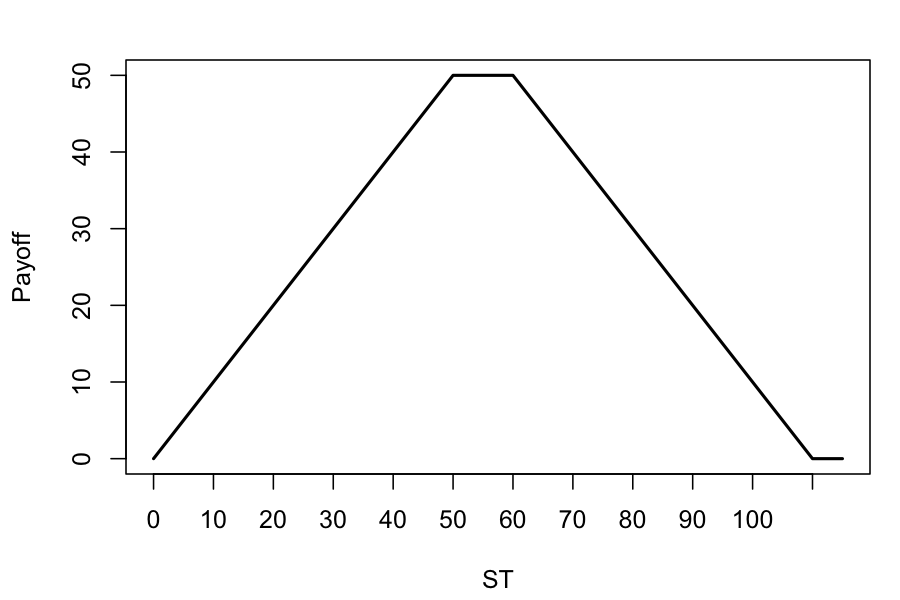
\includegraphics[width=0.55\linewidth]{hw7_graph.png}
    \end{figure}
\end{parts}

\begin{solution}
\begin{parts}
    \part By Put-Call Parity:
    \[
    S_T + \max(E - S_T, 0) = \max(S_T, E) = E + \max(S_T - E, 0)
    \]
    Thus, a protective put (Long Stock $+$ Long Put with strike $E$) has the exact same payoff at expiration as a Long Call (strike $E$) plus a risk-free zero-coupon bond paying face value $E$ at expiration, that is, a fiduciary call. The bond is essential: a long call on its own is not equivalent, since it pays nothing when $S_T < E$ whereas the protective put pays $E$.

    In terms of the parity equation $P + S_0 = C + E e^{-rt}$, the left side is the protective put and the right side is the call plus $E e^{-rt}$ invested at the risk-free rate, which grows to exactly $E$ by expiration.

\begin{lstlisting}[language=R]
ST <- seq(0, 100, by = 0.5)
E <- 50

stock <- ST
put   <- pmax(E - ST, 0)
prot  <- stock + put             # protective put payoff
fiduc <- pmax(ST - E, 0) + E     # long call plus a bond worth E at expiry

par(mfrow = c(1, 2))
plot(ST, prot, type = "l", col = "black", lwd = 3, ylim = c(0, 100),
     xlab = "ST", ylab = "Payoff", main = "Protective put")
lines(ST, stock, col = "red", lty = 2)
lines(ST, put, col = "blue", lty = 2)
abline(h = 0, lty = 2, col = "gray")
legend("topleft", legend = c("long stock", "long put", "protective put"),
       col = c("red", "blue", "black"), lty = c(2, 2, 1), lwd = c(1, 1, 3),
       bty = "n", cex = 0.8)

plot(ST, fiduc, type = "l", col = "darkgreen", lwd = 4, ylim = c(0, 100),
     xlab = "ST", ylab = "Payoff", main = "Long call + bond")
lines(ST, prot, col = "black", lty = 3, lwd = 2)
lines(ST, pmax(ST - E, 0), col = "blue", lty = 2)
abline(h = E, col = "red", lty = 2)
legend("topleft", legend = c("long call", "bond paying E", "call + bond",
                             "protective put"),
       col = c("blue", "red", "darkgreen", "black"), lty = c(2, 2, 1, 3),
       lwd = c(1, 1, 4, 2), bty = "n", cex = 0.8)
\end{lstlisting}

    \begin{figure}[H]
        \centering
        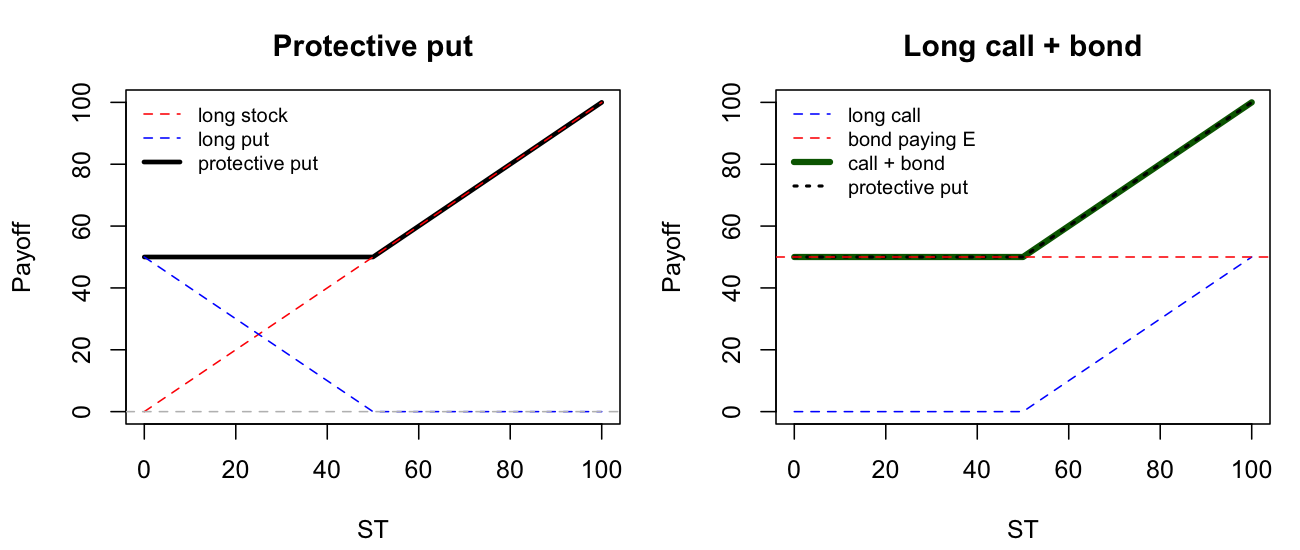
\includegraphics[width=\linewidth]{hw7_ex1a.png}
    \end{figure}

    The two panels are the same function $\max(S_T, E)$, which is what makes the positions equivalent.

    \part The payoff function is:
    \[
    \text{Payoff}(S_T) =
    \begin{cases}
    S_T, & 0 \le S_T \le 50 \\
    50, & 50 < S_T \le 60 \\
    50 - (S_T - 60) = 110 - S_T, & 60 < S_T \le 110 \\
    0, & S_T \ge 110
    \end{cases}
    \]
    We construct this using changes in slopes at $S_T = 0, 50, 60, 110$:
    \begin{itemize}
        \item Initial slope $+1$ starting at $S_T = 0$: buy 1 share of stock ($+S_T$).
        \item Slope changes from $+1$ to $0$ at $S_T = 50$: sell 1 call with $E = 50$ ($-\max(S_T - 50, 0)$).
        \item Slope changes from $0$ to $-1$ at $S_T = 60$: sell 1 call with $E = 60$ ($-\max(S_T - 60, 0)$).
        \item Slope changes from $-1$ to $0$ at $S_T = 110$: buy 1 call with $E = 110$ ($+\max(S_T - 110, 0)$).
    \end{itemize}
    Portfolio composition:
    \[
    \boxed{+1\text{ Stock} - 1\text{ Call }(E=50) - 1\text{ Call }(E=60) + 1\text{ Call }(E=110)}
    \]

\begin{lstlisting}[language=R]
ST <- seq(0, 140, by = 0.5)

stock   <- ST
short50 <- -pmax(ST - 50, 0)
short60 <- -pmax(ST - 60, 0)
long110 <-  pmax(ST - 110, 0)
total   <- stock + short50 + short60 + long110

plot(ST, total, type = "l", col = "black", lwd = 3, ylim = c(-90, 140),
     xlab = "ST", ylab = "Payoff",
     main = "Stock - call(50) - call(60) + call(110)")
lines(ST, stock,   col = "red",       lty = 2)
lines(ST, short50, col = "blue",      lty = 2)
lines(ST, short60, col = "darkgreen", lty = 2)
lines(ST, long110, col = "purple",    lty = 2)
abline(h = 0, lty = 2, col = "gray")
legend("bottomleft",
       legend = c("long stock", "short call E=50", "short call E=60",
                  "long call E=110", "total"),
       col = c("red", "blue", "darkgreen", "purple", "black"),
       lty = c(2, 2, 2, 2, 1), lwd = c(1, 1, 1, 1, 3), bty = "n", cex = 0.8)
\end{lstlisting}

    \begin{figure}[H]
        \centering
        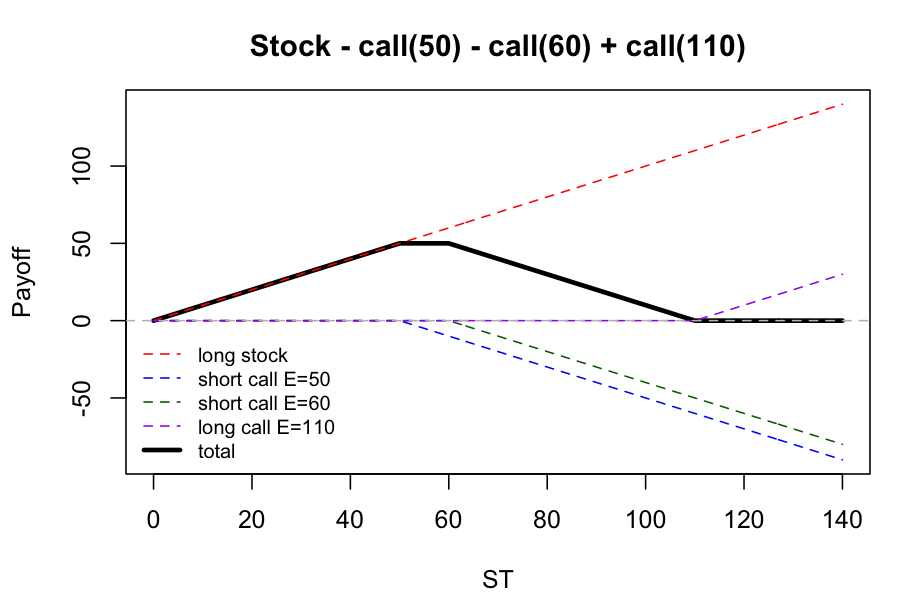
\includegraphics[width=0.75\linewidth]{hw7_ex1b.png}
    \end{figure}
\end{parts}
\end{solution}

\question Answer the following questions:
\begin{parts}
    \part Suppose data are collected for a certain stock:
    \begin{table}[H]
        \centering
        \begin{tabular}{ll}
            Stock price & \$110 \\
            Call price (1-year expiration, $E = \$105$) & \$17 \\
            Put price (1-year expiration, $E = \$105$) & \$5 \\
            Risk-free interest rate & $5\%$ per year \\
        \end{tabular}
    \end{table}
    Is there a mispricing of the call and put? If yes, can you exploit this mispricing to create arbitrage profit? Please provide the numerical example.

    \part The price of a European put option on stock A is \$4.0. The current price of the stock is $S_0 = \$46$. The exercise price of the put option is $E = \$51$, time to expiration is 1 month, and the risk-free interest rate for the one-month period is $0.005$. Is there an opportunity for riskless profit? If there is, please explain the positions you need to hold with the corresponding payoffs.
\end{parts}

\begin{solution}
\begin{parts}
    \part By Put-Call Parity with continuous compounding ($r = 0.05, t = 1$):
    \begin{align*}
    S_0 + P &= 110 + 5 = 115 \\
    C + E e^{-rt} &= 17 + 105 e^{-0.05} \approx 17 + 105(0.951229) = 17 + 99.88 = 116.88
    \end{align*}
    (Or with annual compounding: $17 + \frac{105}{1.05} = 17 + 100 = 117$.)\\
    Since $C + E e^{-rt} > S_0 + P$, the call is overpriced relative to the put. We sell the expensive side and buy the cheap side.

    Arbitrage strategy at $t = 0$:
    \begin{itemize}
        \item Sell Call: $+17$
        \item Buy Put: $-5$
        \item Buy Stock: $-110$
        \item Borrow $E e^{-rt} = \$99.88$ (or $\$100$): $+99.88$
        \item Initial arbitrage profit: $17 - 5 - 110 + 99.88 = \$1.88$ (or $\$2.00$).
    \end{itemize}
    Payoff at expiration $t = 1$:
    \begin{itemize}
        \item Payoff from Stock $+$ Put $-$ Call: $\max(S_1, 105) - \max(S_1 - 105, 0) = 105$.
        \item Repay loan: $-105$.
        \item Net cash flow at $t = 1$: $105 - 105 = \$0$.
    \end{itemize}
    The position costs nothing to unwind in every state of the world, so the \$1.88 collected at $t = 0$ is a riskless profit.

    \part A European put must satisfy the lower bound $P \ge E e^{-rt} - S_0$. Using continuous compounding with $rt = 0.005$ for the one-month period:
    \[
    E e^{-rt} - S_0 = 51 e^{-0.005} - 46 \approx 50.7456 - 46 = \$4.7456
    \]
    Since $P = \$4.00 < \$4.7456$, the put is underpriced relative to its lower bound.

    Arbitrage strategy at $t = 0$:
    \begin{itemize}
        \item Buy Put: $-\$4.00$
        \item Buy Stock: $-\$46.00$
        \item Borrow $S_0 + P = \$50.00$ for one month: $+\$50.00$
        \item Net initial cash flow $= \$0$.
    \end{itemize}
    Payoff at expiration ($t = 1$ month):
    \begin{itemize}
        \item Payoff from Stock $+$ Put $= \max(S_T, 51) \ge 51$.
        \item Repay loan $= 50\,e^{0.005} = \$50.2506$.
        \item Net payoff $= \max(S_T, 51) - 50.2506 \ge 51 - 50.2506 = +\$0.7494 > 0$.
    \end{itemize}
    The position is entered for nothing and can never lose, so this guarantees a riskless profit of at least \$0.7494. (With simple monthly discounting the loan repays \$50.25 and the floor is \$0.75, essentially the same.)
\end{parts}
\end{solution}

\question An investor sells a European call on a share for \$4. The stock price is \$47 and the exercise price is \$50. When does the investor make a profit? When will the option be exercised? Use R to draw a diagram showing the investor's profit against the price of the stock at expiration.

\begin{solution}
Short call: premium received $=\$4$, strike $E = \$50$.
\begin{itemize}
    \item Option exercise: the option is exercised by the buyer whenever $S_T > E$, so for $S_T > 50$.
    \item Profit condition: profit is $4 - \max(S_T - 50, 0)$. The investor makes a profit whenever $4 - (S_T - 50) > 0 \implies S_T < 54$.
    \item Between $S_T = 50$ and $S_T = 54$ the option is exercised but the writer is still ahead. The maximum profit is \$4, and the loss is unbounded above \$54.
\end{itemize}

\begin{lstlisting}[language=R]
ST <- seq(30, 70, by = 0.5)
profit <- 4 - pmax(ST - 50, 0)

plot(ST, profit, type = "l", col = "blue", lwd = 2,
     xlab = "Stock Price at Expiration (ST)", ylab = "Profit ($)",
     main = "Short Call Profit (E = 50, C = 4)")
abline(h = 0, lty = 2, col = "gray")
abline(v = c(50, 54), lty = 3, col = "red")
points(54, 0, pch = 19, col = "red")
text(54, 0.8, "Breakeven = 54", col = "red", pos = 4)
\end{lstlisting}

\begin{figure}[H]
    \centering
    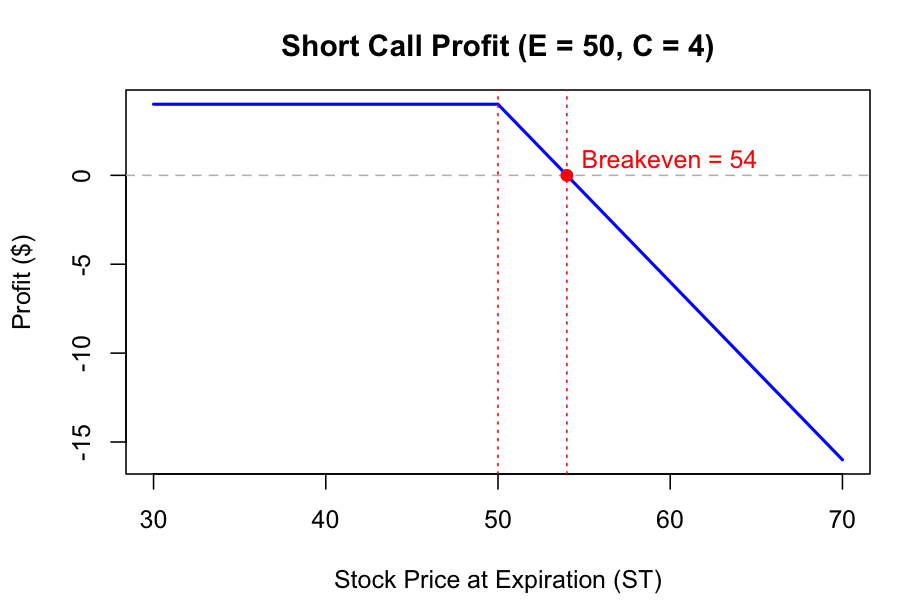
\includegraphics[width=0.7\linewidth]{hw7_ex3.png}
\end{figure}
\end{solution}

\question An investor buys a European put on a share for \$3. The stock price is \$42 and the exercise price is \$40. When does the investor make a profit? When will the option be exercised? Use R to draw a diagram showing the investor's profit against the price of the stock at expiration.

\begin{solution}
Long put: premium paid $=\$3$, strike $E = \$40$.
\begin{itemize}
    \item Option exercise: the option is exercised whenever $S_T < E$, so for $S_T < 40$.
    \item Profit condition: profit is $\max(40 - S_T, 0) - 3$. The investor makes a profit when $(40 - S_T) - 3 > 0 \implies S_T < 37$.
    \item Between $S_T = 37$ and $S_T = 40$ the option is exercised but the premium is not fully recovered. The loss is capped at the \$3 premium and the maximum profit is \$37 at $S_T = 0$.
\end{itemize}

\begin{lstlisting}[language=R]
ST <- seq(20, 60, by = 0.5)
profit <- pmax(40 - ST, 0) - 3

plot(ST, profit, type = "l", col = "darkgreen", lwd = 2,
     xlab = "Stock Price at Expiration (ST)", ylab = "Profit ($)",
     main = "Long Put Profit (E = 40, P = 3)")
abline(h = 0, lty = 2, col = "gray")
abline(v = c(40, 37), lty = 3, col = "red")
points(37, 0, pch = 19, col = "red")
text(37, 0.8, "Breakeven = 37", col = "red", pos = 2)
\end{lstlisting}

\begin{figure}[H]
    \centering
    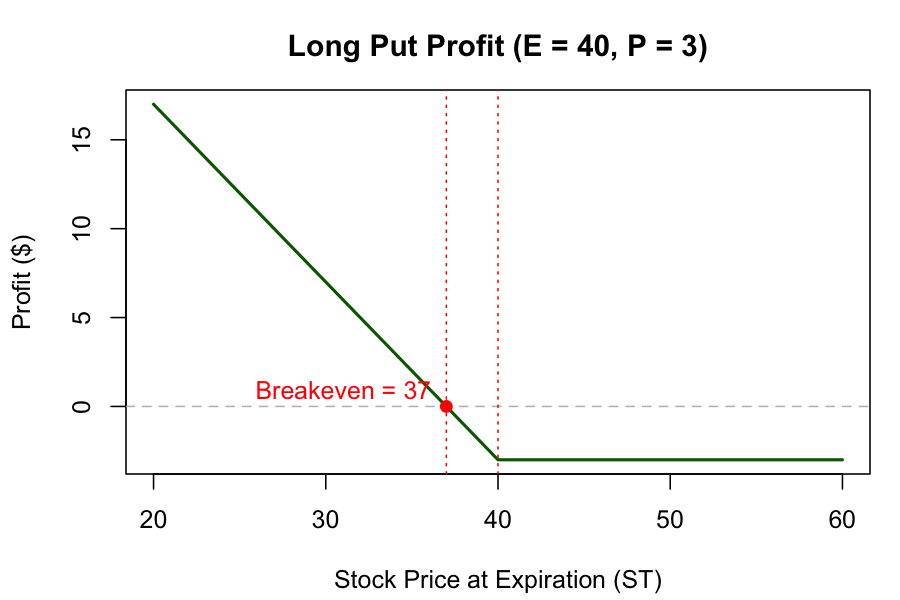
\includegraphics[width=0.7\linewidth]{hw7_ex4.png}
\end{figure}
\end{solution}

\question You want to purchase 2 puts and 1 call. The call option costs \$5 and the put option costs \$6. The exercise price for the call or the put is \$50. Use R to plot the profit against the stock price at the expiration date:
\begin{parts}
    \part For the 2 puts.
    \part For the call.
    \part For the combination of the 2 puts and 1 call.
\end{parts}

\begin{solution}
Total premium paid:
\begin{itemize}
    \item 2 Puts: $2 \times 6 = \$12$
    \item 1 Call: $\$5$
    \item Total: $\$17$
\end{itemize}
Two puts and one call at a common strike is a strip, which profits from a large move in either direction but twice as fast on the downside. Break-even points:
\begin{itemize}
    \item (a) 2 puts: $2(50 - S_T) = 12 \implies S_T = 44$.
    \item (b) 1 call: $S_T - 50 = 5 \implies S_T = 55$.
    \item (c) combination: $2(50 - S_T) = 17 \implies S_T = 41.5$ on the downside, and $S_T - 50 = 17 \implies S_T = 67$ on the upside.
\end{itemize}

\begin{lstlisting}[language=R]
ST <- seq(20, 80, by = 0.5)
profit_puts  <- 2 * pmax(50 - ST, 0) - 12
profit_call  <- pmax(ST - 50, 0) - 5
profit_total <- profit_puts + profit_call

par(mfrow = c(2, 2))

# (a) the two puts
plot(ST, profit_puts, type = "l", col = "red", lwd = 2,
     xlab = "ST", ylab = "Profit ($)", main = "(a) 2 Long Puts (E = 50)")
abline(h = 0, lty = 2, col = "gray"); abline(v = 44, lty = 3, col = "red")

# (b) the call
plot(ST, profit_call, type = "l", col = "blue", lwd = 2,
     xlab = "ST", ylab = "Profit ($)", main = "(b) 1 Long Call (E = 50)")
abline(h = 0, lty = 2, col = "gray"); abline(v = 55, lty = 3, col = "red")

# (c) the combination
plot(ST, profit_total, type = "l", col = "purple", lwd = 2, ylim = c(-20, 70),
     xlab = "ST", ylab = "Profit ($)", main = "(c) Strip: 2 Puts + 1 Call")
lines(ST, profit_puts, col = "red", lty = 2)
lines(ST, profit_call, col = "blue", lty = 2)
abline(h = 0, lty = 2, col = "gray")
abline(v = c(41.5, 67), lty = 3, col = "red")
legend("top", legend = c("Combined", "2 Puts", "1 Call"),
       col = c("purple", "red", "blue"), lty = c(1, 2, 2), lwd = 2,
       bty = "n", cex = 0.8)
\end{lstlisting}

\begin{figure}[H]
    \centering
    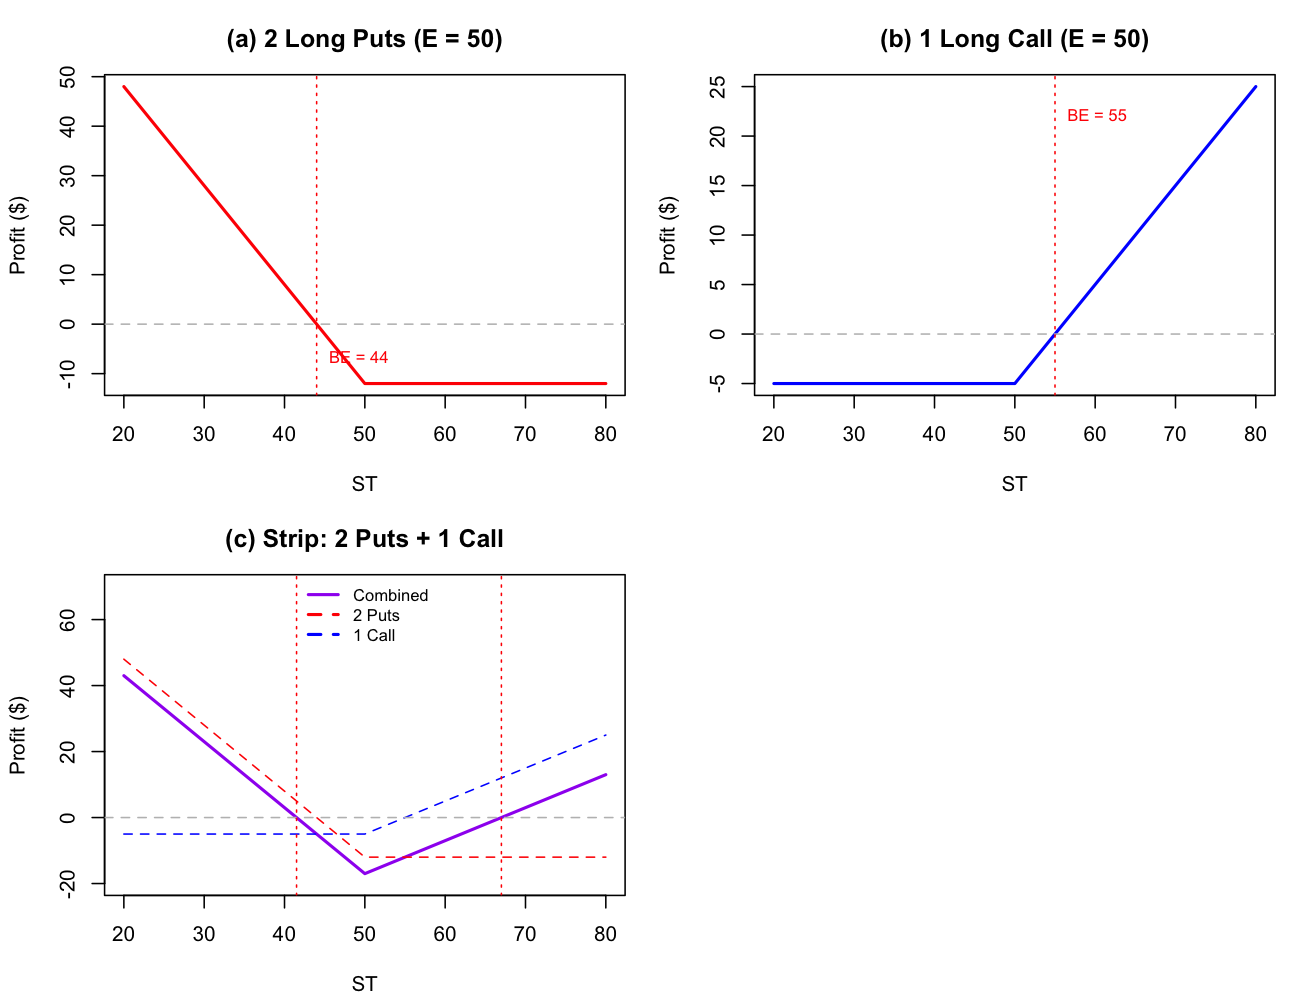
\includegraphics[width=\linewidth]{hw7_ex5.png}
\end{figure}
\end{solution}

\question Consider the following strategy: You write 2 call options (each one with $E = \$45$, $C = \$5$) and you buy 1 call option (with $E = \$40$, $C = \$8$). Both buying and selling call options have the same expiration date. Use R to plot the profit against the stock price at the expiration date for this strategy.

\begin{solution}
Net premium received: $2(5) - 8 = +\$2$.
\[
\text{Profit}(S_T) = \max(S_T - 40, 0) - 2\max(S_T - 45, 0) + 2
\]
This is a ratio call spread. The profit is \$2 for $S_T \le 40$, rises to a maximum of \$7 at $S_T = 45$, and then falls one for one, crossing zero at $S_T = 52$. Because two calls are written against only one held, the loss above \$52 is unbounded.

\begin{lstlisting}[language=R]
ST <- seq(25, 65, by = 0.5)
profit <- pmax(ST - 40, 0) - 2 * pmax(ST - 45, 0) + 2

plot(ST, profit, type = "l", col = "blue", lwd = 2,
     xlab = "Stock Price at Expiration (ST)", ylab = "Profit ($)",
     main = "Buy 1 Call (E=40) + Sell 2 Calls (E=45)")
abline(h = 0, lty = 2, col = "gray")
abline(v = c(40, 45, 52), lty = 3, col = "red")
points(52, 0, pch = 19, col = "red")
text(52, 0.8, "Breakeven = 52", col = "red", pos = 4)
\end{lstlisting}

\begin{figure}[H]
    \centering
    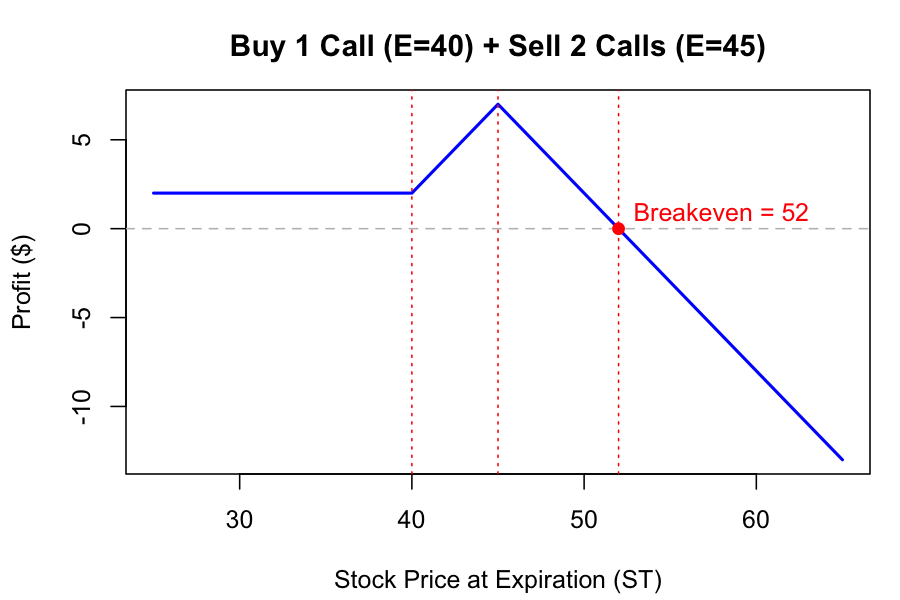
\includegraphics[width=0.7\linewidth]{hw7_ex6.png}
\end{figure}
\end{solution}

\question By rearranging the put call parity equation $P + S_0 = C + E e^{-rt}$ give an example in R to show the payoff and profit using the following investing strategies:
\begin{parts}
    \part Long put long stock.
    \part Short put short stock.
    \part Long call short stock.
    \part Short call long stock.
\end{parts}

\begin{solution}
Take $S_0 = 50$, $E = 50$, $C = 5$ and $r = 0$, so that $E e^{-rt} = E = 50$ and parity gives $P = C + E e^{-rt} - S_0 = 5$. Setting $r = 0$ is what makes $C = P = 5$ consistent with parity at $S_0 = E$; with a positive rate the two premiums could not both be \$5.

The four rearrangements are
\begin{align*}
\text{(a)}\quad P + S_0 &= C + E e^{-rt} & &\text{payoff } \max(S_T, E)\\
\text{(b)}\quad -P - S_0 &= -C - E e^{-rt} & &\text{payoff } -\max(S_T, E)\\
\text{(c)}\quad C - S_0 &= P - E e^{-rt} & &\text{payoff } -\min(S_T, E)\\
\text{(d)}\quad S_0 - C &= E e^{-rt} - P & &\text{payoff } \min(S_T, E)
\end{align*}

\begin{lstlisting}[language=R]
ST <- seq(20, 80, by = 0.5)
S0 <- 50; E <- 50; C <- 5; P <- 5   # r = 0, so PV(E) = E and parity holds

par(mfrow = c(2, 2))

# (a) long put + long stock = long call + bond
payoff_a <- ST + pmax(E - ST, 0)
profit_a <- payoff_a - (S0 + P)
plot(ST, payoff_a, type = "l", col = "blue", lwd = 3, ylim = c(-40, 100),
     main = "(a) Long Put + Long Stock", xlab = "ST", ylab = "Payoff / Profit")
lines(ST, pmax(ST - E, 0) + E, col = "darkgreen", lty = 3, lwd = 2)
lines(ST, profit_a, col = "red", lwd = 2)
abline(h = 0, lty = 2, col = "gray")

# (b) short put + short stock
payoff_b <- -payoff_a
profit_b <- payoff_b + (S0 + P)
plot(ST, payoff_b, type = "l", col = "blue", lwd = 3, ylim = c(-100, 40),
     main = "(b) Short Put + Short Stock", xlab = "ST", ylab = "Payoff / Profit")
lines(ST, -(pmax(ST - E, 0) + E), col = "darkgreen", lty = 3, lwd = 2)
lines(ST, profit_b, col = "red", lwd = 2)
abline(h = 0, lty = 2, col = "gray")

# (c) long call + short stock = long put + borrow PV(E)
payoff_c <- pmax(ST - E, 0) - ST
profit_c <- payoff_c + (S0 - C)
plot(ST, payoff_c, type = "l", col = "blue", lwd = 3, ylim = c(-80, 20),
     main = "(c) Long Call + Short Stock", xlab = "ST", ylab = "Payoff / Profit")
lines(ST, pmax(E - ST, 0) - E, col = "darkgreen", lty = 3, lwd = 2)
lines(ST, profit_c, col = "red", lwd = 2)
abline(h = 0, lty = 2, col = "gray")

# (d) short call + long stock = bond + short put (covered call)
payoff_d <- ST - pmax(ST - E, 0)
profit_d <- payoff_d - (S0 - C)
plot(ST, payoff_d, type = "l", col = "blue", lwd = 3, ylim = c(-20, 80),
     main = "(d) Short Call + Long Stock", xlab = "ST", ylab = "Payoff / Profit")
lines(ST, E - pmax(E - ST, 0), col = "darkgreen", lty = 3, lwd = 2)
lines(ST, profit_d, col = "red", lwd = 2)
abline(h = 0, lty = 2, col = "gray")
\end{lstlisting}

\begin{figure}[H]
    \centering
    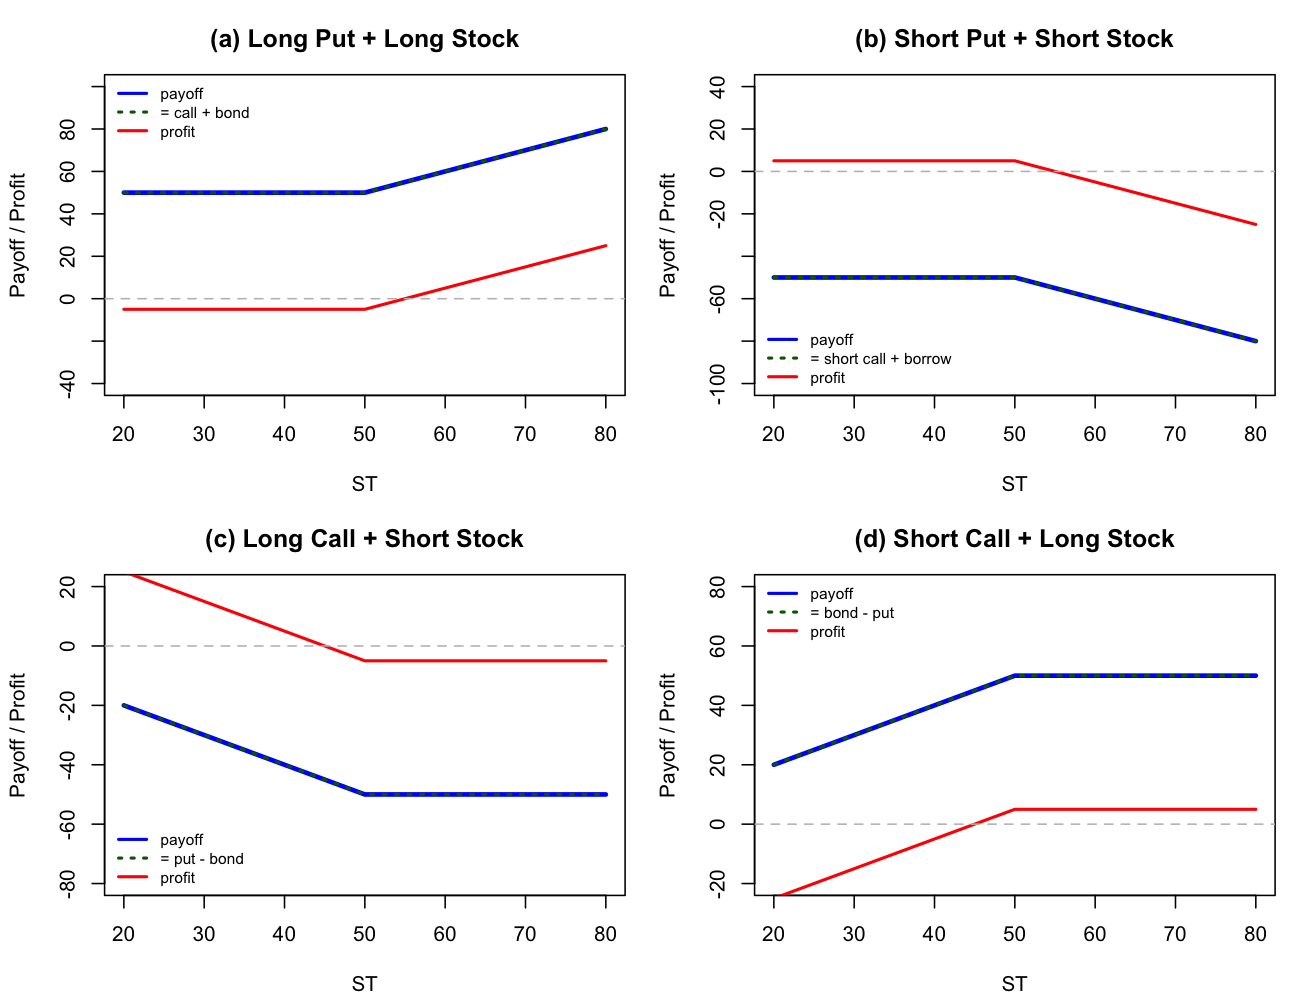
\includegraphics[width=\linewidth]{hw7_ex7.png}
\end{figure}

In every panel the solid payoff line and the dotted line from the other side of the parity equation coincide exactly, which is the content of put-call parity. The profit line is the payoff shifted down by the net cost of setting up the position.
\end{solution}

\question Consider the box spread strategy: It is a combination of a bull call spread and a bear put spread.
\begin{itemize}
    \item Bull call spread: Buy one call with exercise $E_1 = \$50$ and sell one call with exercise $E_2 = \$60$.
    \item Bear put spread: Buy one put with exercise $E_2 = \$60$ and sell one put with exercise $E_1 = \$50$.
\end{itemize}
\begin{parts}
    \part Complete the table that shows the payoffs for all the positions above.
    \part Construct the diagram in R that shows the payoff for the bull call spread, for the bear put spread, and the total.
\end{parts}

\begin{solution}
\begin{parts}
    \part Payoff table at expiration:
    \begin{table}[H]
        \centering
        \begin{tabular}{lccc}
            \hline
            Position & $S_T \le 50$ & $50 < S_T < 60$ & $S_T \ge 60$ \\
            \hline
            Buy Call ($E_1 = 50$) & $0$ & $S_T - 50$ & $S_T - 50$ \\
            Sell Call ($E_2 = 60$) & $0$ & $0$ & $-(S_T - 60)$ \\
            Bull Call Spread & $0$ & $S_T - 50$ & $10$ \\
            \hline
            Buy Put ($E_2 = 60$) & $60 - S_T$ & $60 - S_T$ & $0$ \\
            Sell Put ($E_1 = 50$) & $-(50 - S_T)$ & $0$ & $0$ \\
            Bear Put Spread & $10$ & $60 - S_T$ & $0$ \\
            \hline
            Total (Box Spread) & $10$ & $10$ & $10$ \\
            \hline
        \end{tabular}
    \end{table}
    The payoff of a box spread is constant: $\boxed{E_2 - E_1 = 10}$ under all conditions. Because the payoff carries no risk, the box is a synthetic zero-coupon bond and must cost $(E_2 - E_1)e^{-rt}$ today; any other price is an arbitrage.

    \part
    \begin{lstlisting}[language=R]
ST <- seq(30, 80, by = 0.5)
bull_call <- pmax(ST - 50, 0) - pmax(ST - 60, 0)
bear_put  <- pmax(60 - ST, 0) - pmax(50 - ST, 0)
total_box <- bull_call + bear_put

plot(ST, total_box, type = "l", col = "purple", lwd = 3, ylim = c(-2, 14),
     xlab = "Stock Price at Expiration (ST)", ylab = "Payoff ($)",
     main = "Box Spread Payoff Diagram")
lines(ST, bull_call, col = "blue", lty = 2, lwd = 1.5)
lines(ST, bear_put, col = "red", lty = 2, lwd = 1.5)
abline(h = 0, lty = 2, col = "gray")
legend("topleft",
       legend = c("Box Spread (Total = 10)", "Bull Call Spread",
                  "Bear Put Spread"),
       col = c("purple", "blue", "red"), lty = c(1, 2, 2), lwd = 2, bty = "n")
    \end{lstlisting}

    \begin{figure}[H]
        \centering
        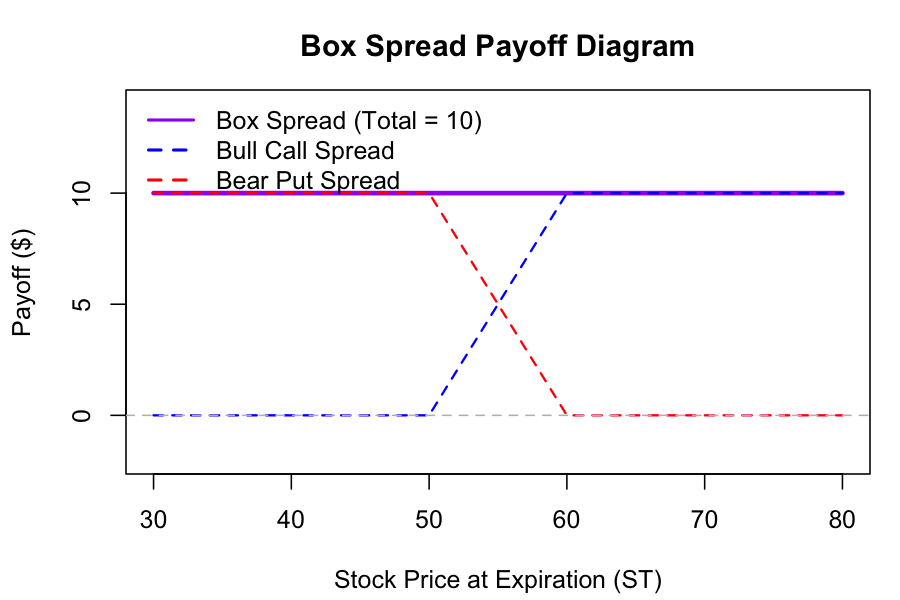
\includegraphics[width=0.7\linewidth]{hw7_ex8.png}
    \end{figure}
\end{parts}
\end{solution}

\question Consider creating a bear spread using puts: Sell one put with exercise $E_1$ and buy one put with exercise price $E_2$, with $E_2 > E_1$. Complete the table that shows the payoff and profit for each position and the total and use a numerical example in R to show the diagram for each position and the total.

\begin{solution}
Let $P_1$ and $P_2$ be the premiums of puts with strikes $E_1$ and $E_2$ ($P_2 > P_1$). Net initial cost is $P_2 - P_1 > 0$.

\begin{table}[H]
    \centering
    \begin{tabular}{lccc}
        \hline
        Position & $S_T \le E_1$ & $E_1 < S_T < E_2$ & $S_T \ge E_2$ \\
        \hline
        Buy Put ($E_2$) Payoff & $E_2 - S_T$ & $E_2 - S_T$ & $0$ \\
        Sell Put ($E_1$) Payoff & $-(E_1 - S_T)$ & $0$ & $0$ \\
        Total Payoff & $E_2 - E_1$ & $E_2 - S_T$ & $0$ \\
        \hline
        Total Profit & $(E_2 - E_1) - (P_2 - P_1)$ & $(E_2 - S_T) - (P_2 - P_1)$ & $-(P_2 - P_1)$ \\
        \hline
    \end{tabular}
\end{table}

With $E_1 = 45$, $E_2 = 55$, $P_1 = 2$ and $P_2 = 6$ the spread costs \$4. The maximum profit is $10 - 4 = \$6$ for $S_T \le 45$, the maximum loss is \$4 for $S_T \ge 55$, and the break-even is at $S_T = E_2 - (P_2 - P_1) = \$51$.

\begin{lstlisting}[language=R]
ST <- seq(30, 70, by = 0.5)
E1 <- 45; E2 <- 55; P1 <- 2; P2 <- 6

payoff_buy   <- pmax(E2 - ST, 0)
payoff_sell  <- -pmax(E1 - ST, 0)
payoff_total <- payoff_buy + payoff_sell
profit_total <- payoff_total - (P2 - P1)

plot(ST, profit_total, type = "l", col = "darkgreen", lwd = 2.5,
     ylim = c(-12, 22),
     xlab = "Stock Price at Expiration (ST)", ylab = "Profit / Payoff ($)",
     main = "Bear Put Spread (E1 = 45, E2 = 55)")
lines(ST, payoff_total, col = "purple", lty = 2, lwd = 1.5)
lines(ST, payoff_buy - P2, col = "blue", lty = 3)
lines(ST, payoff_sell + P1, col = "red", lty = 3)
abline(h = 0, lty = 2, col = "gray")
abline(v = E2 - (P2 - P1), lty = 3, col = "gray40")
legend("topright",
       legend = c("Total Profit", "Total Payoff", "Long Put Profit",
                  "Short Put Profit"),
       col = c("darkgreen", "purple", "blue", "red"), lty = c(1, 2, 3, 3),
       lwd = 2, bty = "n", cex = 0.85)
\end{lstlisting}

\begin{figure}[H]
    \centering
    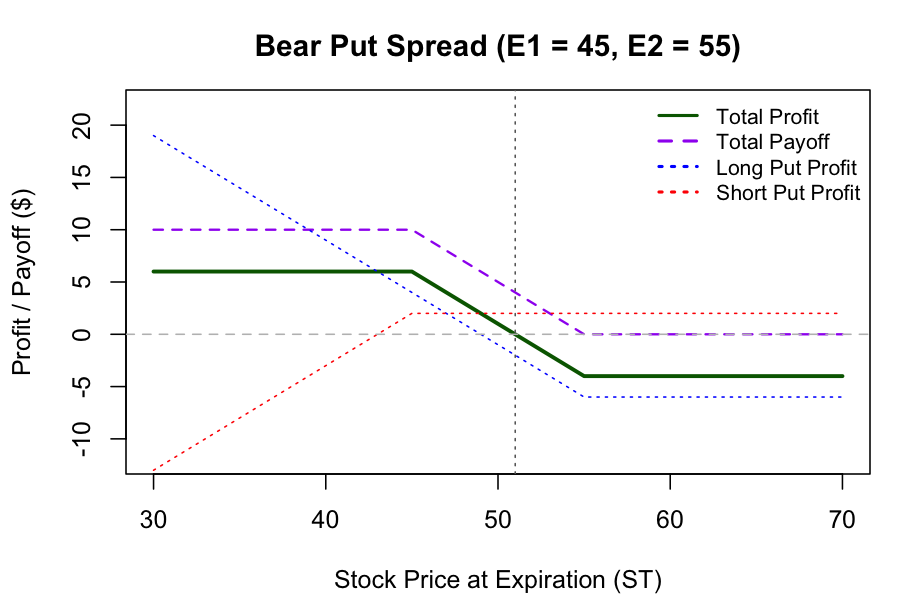
\includegraphics[width=0.7\linewidth]{hw7_ex9.png}
\end{figure}
\end{solution}

\question Consider creating a bear spread using calls: Sell one call with exercise $E_1$ and buy one call with exercise price $E_2$, with $E_2 > E_1$. Complete the table that shows the payoff and profit for each position and the total and use a numerical example in R to show the diagram for each position and the total.

\begin{solution}
Let $C_1$ and $C_2$ be the premiums of calls with strikes $E_1$ and $E_2$ ($C_1 > C_2$). Net initial cash inflow is $C_1 - C_2 > 0$.

\begin{table}[H]
    \centering
    \begin{tabular}{lccc}
        \hline
        Position & $S_T \le E_1$ & $E_1 < S_T < E_2$ & $S_T \ge E_2$ \\
        \hline
        Sell Call ($E_1$) Payoff & $0$ & $-(S_T - E_1)$ & $-(S_T - E_1)$ \\
        Buy Call ($E_2$) Payoff & $0$ & $0$ & $S_T - E_2$ \\
        Total Payoff & $0$ & $-(S_T - E_1)$ & $-(E_2 - E_1)$ \\
        \hline
        Total Profit & $C_1 - C_2$ & $(C_1 - C_2) - (S_T - E_1)$ & $(C_1 - C_2) - (E_2 - E_1)$ \\
        \hline
    \end{tabular}
\end{table}

With $E_1 = 45$, $E_2 = 55$, $C_1 = 7$ and $C_2 = 2$ the spread is opened for a \$5 credit. The maximum profit is \$5 for $S_T \le 45$, the maximum loss is $10 - 5 = \$5$ for $S_T \ge 55$, and the break-even is at $S_T = E_1 + (C_1 - C_2) = \$50$.

\begin{lstlisting}[language=R]
ST <- seq(30, 70, by = 0.5)
E1 <- 45; E2 <- 55; C1 <- 7; C2 <- 2

payoff_sell  <- -pmax(ST - E1, 0)
payoff_buy   <- pmax(ST - E2, 0)
payoff_total <- payoff_sell + payoff_buy
profit_total <- payoff_total + (C1 - C2)

plot(ST, profit_total, type = "l", col = "darkred", lwd = 2.5,
     ylim = c(-22, 12),
     xlab = "Stock Price at Expiration (ST)", ylab = "Profit / Payoff ($)",
     main = "Bear Call Spread (E1 = 45, E2 = 55)")
lines(ST, payoff_total, col = "purple", lty = 2, lwd = 1.5)
lines(ST, payoff_sell + C1, col = "red", lty = 3)
lines(ST, payoff_buy - C2, col = "blue", lty = 3)
abline(h = 0, lty = 2, col = "gray")
abline(v = E1 + (C1 - C2), lty = 3, col = "gray40")
legend("topright",
       legend = c("Total Profit", "Total Payoff", "Short Call Profit",
                  "Long Call Profit"),
       col = c("darkred", "purple", "red", "blue"), lty = c(1, 2, 3, 3),
       lwd = 2, bty = "n", cex = 0.85)
\end{lstlisting}

\begin{figure}[H]
    \centering
    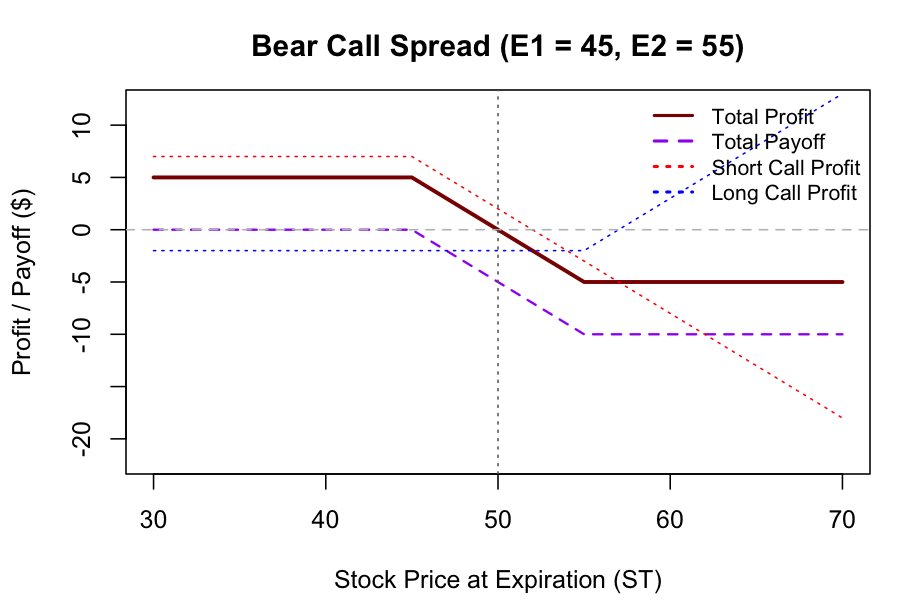
\includegraphics[width=0.7\linewidth]{hw7_ex10.png}
\end{figure}
\end{solution}

\end{questions}

\end{document}
